% Options for packages loaded elsewhere
\PassOptionsToPackage{unicode}{hyperref}
\PassOptionsToPackage{hyphens}{url}
\documentclass[
]{article}
\usepackage{xcolor}
\usepackage{amsmath,amssymb}
\setcounter{secnumdepth}{-\maxdimen} % remove section numbering
\usepackage{iftex}
\ifPDFTeX
  \usepackage[T1]{fontenc}
  \usepackage[utf8]{inputenc}
  \usepackage{textcomp} % provide euro and other symbols
\else % if luatex or xetex
  \usepackage{unicode-math} % this also loads fontspec
  \defaultfontfeatures{Scale=MatchLowercase}
  \defaultfontfeatures[\rmfamily]{Ligatures=TeX,Scale=1}
\fi
\usepackage{lmodern}
\ifPDFTeX\else
  % xetex/luatex font selection
\fi
% Use upquote if available, for straight quotes in verbatim environments
\IfFileExists{upquote.sty}{\usepackage{upquote}}{}
\IfFileExists{microtype.sty}{% use microtype if available
  \usepackage[]{microtype}
  \UseMicrotypeSet[protrusion]{basicmath} % disable protrusion for tt fonts
}{}
\makeatletter
\@ifundefined{KOMAClassName}{% if non-KOMA class
  \IfFileExists{parskip.sty}{%
    \usepackage{parskip}
  }{% else
    \setlength{\parindent}{0pt}
    \setlength{\parskip}{6pt plus 2pt minus 1pt}}
}{% if KOMA class
  \KOMAoptions{parskip=half}}
\makeatother
\usepackage{graphicx}
\makeatletter
\newsavebox\pandoc@box
\newcommand*\pandocbounded[1]{% scales image to fit in text height/width
  \sbox\pandoc@box{#1}%
  \Gscale@div\@tempa{\textheight}{\dimexpr\ht\pandoc@box+\dp\pandoc@box\relax}%
  \Gscale@div\@tempb{\linewidth}{\wd\pandoc@box}%
  \ifdim\@tempb\p@<\@tempa\p@\let\@tempa\@tempb\fi% select the smaller of both
  \ifdim\@tempa\p@<\p@\scalebox{\@tempa}{\usebox\pandoc@box}%
  \else\usebox{\pandoc@box}%
  \fi%
}
% Set default figure placement to htbp
\def\fps@figure{htbp}
\makeatother
\setlength{\emergencystretch}{3em} % prevent overfull lines
\providecommand{\tightlist}{%
  \setlength{\itemsep}{0pt}\setlength{\parskip}{0pt}}
\usepackage{bookmark}
\IfFileExists{xurl.sty}{\usepackage{xurl}}{} % add URL line breaks if available
\urlstyle{same}
\hypersetup{
  hidelinks,
  pdfcreator={LaTeX via pandoc}}

\author{}
\date{}

\begin{document}

{}

{SISTEMI VIRTUALIZZATI}

{}

{}

{}

\section{\texorpdfstring{{Virtualizzazione}}{Virtualizzazione}}\label{h.8tyq566c7yxy}

{}

{È l'astrazione dei componenti hardware di elaboratori per renderli
disponibili, come risorsa virtuale, al software.}

{}

{In questo modo è possibile installare S.O. su hardware virtuale,
l\textquotesingle insieme di questo hardware è detto Virtual Machine.}

\subsection{\texorpdfstring{{Vantaggi}}{Vantaggi}}\label{h.icgp4fuvi9em}

\begin{itemize}
\tightlist
\item
  {Utilizzo superiore dell'hardware;}
\end{itemize}

{}

\begin{itemize}
\tightlist
\item
  {Riduzione consumi e spazio;}
\end{itemize}

{}

\begin{itemize}
\tightlist
\item
  {Isolamento sistemi;}
\end{itemize}

{}

\begin{itemize}
\tightlist
\item
  {Più S.O. nello stesso hardware;}
\end{itemize}

{}

\begin{itemize}
\tightlist
\item
  {Gestione, portabilità e scalabilità migliore.}
\end{itemize}

\subsection{\texorpdfstring{{Terminologia}}{Terminologia}}\label{h.29k94dsrwn6p}

\begin{itemize}
\tightlist
\item
  {Host}{: macchina fisica dove gir}{a}{~il S.O. principale, dove si
  ospitano le macchine virtuali;}
\end{itemize}

{}

\begin{itemize}
\tightlist
\item
  {Guest}{: è la macchina virtuale, si trova ``sopra'' l'host;}
\end{itemize}

{}

\begin{itemize}
\tightlist
\item
  {Hypervisor}{: detto anche virtual machine monitor è quel software che
  avvia e crea le VM.}
\end{itemize}

\subsection{\texorpdfstring{{Tipi di
virtualizzazione}}{Tipi di virtualizzazione}}\label{h.6hzz4zvpzhiw}

\begin{itemize}
\tightlist
\item
  {Virt. Desktop}{: l'utente crea una macchina virtuale sulla propria
  macchina fisica tramite un hypervisor di tipo 2 (hosted), per accedere
  alla VM l'utente utilizza le periferiche della propria macchina
  fisica. Utile per utilizzare software non compatibile sulla propria
  macchina;}
\end{itemize}

{}

\begin{itemize}
\tightlist
\item
  {Virt. Server}{: si realizza una VM in un data center tramite S.O.
  dedicati e hypervisor di tipo 1 (bare-metal) permettendo di eseguire
  altri S.O. direttamente sull'hardware, l'utente ci accedere da
  remoto;}
\end{itemize}

{}

\begin{itemize}
\tightlist
\item
  {{[}...{]}}{~CPU}{: dobbiamo distinguere fra:}
\end{itemize}

{}

\begin{enumerate}
\tightlist
\item
  {Virtualizzazione}{:}{~si crea una CPU virtuale che esegue lo stesso
  tipo di istruzioni macchina della CPU reale. La CPU virtuale quindi
  può fare eseguire le istruzioni dei programmi direttamente dalla CPU
  reale}{;}
\end{enumerate}

{}

\begin{enumerate}
\setcounter{enumi}{1}
\tightlist
\item
  {Emulazione}{:}{~si costruisce una CPU virtuale che esegue istruzioni
  di tipo diverso da quello della CPU reale, quindi le istruzioni devono
  essere tradotte in istruzioni macchina.}
\end{enumerate}

{}

\subsection{\texorpdfstring{{Protection
Ring}}{Protection Ring}}\label{h.q8pjxvtrenj9}

{Sono 4 ``anelli'' di protezione per le CPU moderne, vanno da 0 a 3
quando la CPU è settata per stare nei rings di livello più }{alto è
abilitata}{~a fare istruzioni non privilegiate.}

{Nei rings più bassi}{~la CPU può fare tutte quelle }{istruzioni più
pericolose}{~tipiche del S.O.}

\subsection{\texorpdfstring{{Virt. livello
HW}}{Virt. livello HW}}\label{h.ipmu7njsj3v2}

{Sono le VM e all\textquotesingle utente del sistema di virtualizzazione
viene presentata un\textquotesingle interfaccia su cui installare un
sistema operativo, quindi una CPU virtuale (ma dello stesso tipo della
CPU fisica) e risorse HW virtuali.}

{I S.O. vengono eseguiti in modo concorrente sullo stesso hardware e
possono solitamente essere eterogenei e l'hypervisor
}{multiplexa}{~l'accesso alle risorse.}

{In questa categoria può capitare che l'hypervisor possa svolgere il
ruolo di S.O. essendo un processo all'interno di un altro S.O.}

{}

\subsubsection{\texorpdfstring{{Virt. tipo 1 e
2}}{Virt. tipo 1 e 2}}\label{h.kefqvre9zyv}

{La virtualizzazione di tipo 1 o }{bare-metal}{~è quando il s.o. host è
assente e l'hypervisor prende il suo posto (virtualizzazione server).}

{}

{La virtualizzazione di tipo 2 o }{hosted}{~è quando un hypervisor è un
processo utente (virtualizzazione desktop).}

{}

{}

\subsubsection{\texorpdfstring{{Full e Para
Virtualization}}{Full e Para Virtualization}}\label{h.cr6tx6bo912l}

{È una suddivisione della virtualizzazione HW:}

{}

\begin{itemize}
\tightlist
\item
  {Para-virtualization}{: la VM presenta un\textquotesingle interfaccia
  differente rispetto ad una macchina fisica. Questo comporta dover
  modificare il sistema operativo guest per consentire
  l\textquotesingle esecuzione all\textquotesingle interno della
  macchina virtuale stessa. Si utilizzano API (}{hypercall}{) per
  permettere al s.o. guest di interfacciarsi e permettere tutte le
  operazioni classiche di un sistema.}
\end{itemize}

{}

\begin{itemize}
\tightlist
\item
  {Full-virtualization}{: le macchine virtuali hanno la stessa
  interfaccia di una fisica, il sistema guest non sa di essere virtuale
  e non c'è bisogno di modificare il }{s.o.}
\end{itemize}

{Per eseguire le istruzioni privilegiate, limitando e controllando le
azioni in modo da evitare problemi, vengono adottate due modalità:}

\begin{enumerate}
\tightlist
\item
  {Binary translation}{: consiste nel scrivere le istruzioni binarie. La
  CPU opera in modalità debug, ad ogni comando sospende l'esecuzione,
  analizza il codice e copia delle parti in una cache dove viene
  modificato per far in modo che il codice lavori sulle risorse della
  VM.}
\end{enumerate}

{}

\begin{enumerate}
\setcounter{enumi}{1}
\tightlist
\item
  {Hardware assisted}{: viene aggiunto un nuovo ring chiamato }{ring
  -1}{, il sistema host e l'hypervisor vengono eseguiti in quest'ultimo
  ring mentre il guest in quello 0.}
\end{enumerate}

{Così facendo il sistema operativo guest può eseguire le istruzioni
privilegiate, sotto però il controllo dell\textquotesingle hypervisor.
}{È possibile annidare più VM una dentro l'altra}{~essendoci più tabelle
con le info su ciascuna VM.}

{}

{Nella para-virtualization questo problema non persiste perchè il
}{s.o.}{~non invoca direttamente le istruzioni privilegiate.}

{}

{}

\subsection{\texorpdfstring{{Virt. livello
OS}}{Virt. livello OS}}\label{h.exro2jxs3nps}

{Sono i container, all\textquotesingle utente viene presentata una
partizione del sistema operativo corrente, su cui installare ed eseguire
applicazioni che}{~rimangono isolate}{~nella partizione, }{pur accedendo
ai servizi di uno stesso }{o.s}{.}

{In questo tipo la virtualizzazione è composta da un solo kernel e
istanze isolate che possono essere modificate e utilizzate
indipendentemente tra loro.}

{}

\subsection{\texorpdfstring{{Container}}{Container}}\label{h.la4f4eujhkv6}

{Creano uno spazio utente isolato (anche se non perfetto), con proprie
librerie e }{file,}{~isolando una applicazione dal resto del sistema
operativo, più container possono appoggiarsi ad uno stesso spazio kernel
e }{usano servizi di uno stesso S.O.}

{Il container offre basso sovraccarico per il content-switching e di
memoria senza la possibilità di usare S.O. differenti.}

{I principali container sono: }

{}

\begin{itemize}
\tightlist
\item
  {Docker}{: si appoggia sul s.o. Linux che fornisce un supporto per
  container detto LXC (Linux Container);}
\end{itemize}

{}

\begin{itemize}
\tightlist
\item
  {Hyper-V}{: proprietario di Microsoft, in realtà si chiamano container
  ma sono delle semplici macchine virtuali;}
\end{itemize}

{}

\begin{itemize}
\tightlist
\item
  {Container di Windows Server}{: sono effettivamente dei container. }
\end{itemize}

{}

{}

\subsubsection{\texorpdfstring{{Docker
Swarm}}{Docker Swarm}}\label{h.w4o7r9679d6h}

{Distribuire il carico su più container e su più macchine.}

{In Docker Swarm esiste un cluster di macchine comandate da un }{nodo
Manager}{~(gli altri nodi sono detti }{worker}{), il}{~nodo Manager
}{distribuisce gli }{insiemi }{(service) e i }{container }{(task) fra i
}{worker}{; i task e i service insieme formano una applicazione.}

{}

{\pandocbounded{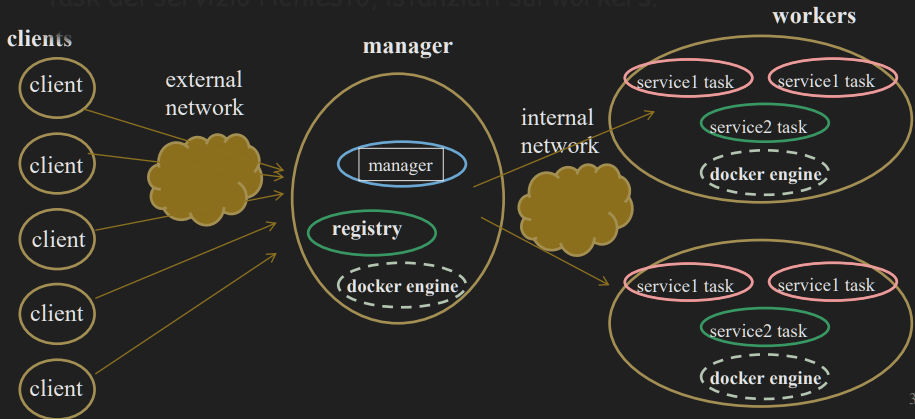
\includegraphics[keepaspectratio]{images/image3.png}}}

{}

{}

{}

\subsubsection{\texorpdfstring{{Kubernetes}}{Kubernetes}}\label{h.n5x6ryfqn2lr}

{Fornisce }{automaticamente scalabilità e resilienza ad applicazioni
basate su container docker, in esecuzione su cluster di host fisici o
virtuali.}

{Le applicazioni progettate per kubernetes sono costituite da più pods,
dove ciascun ~pods è un insieme di container che cooperano e comunicano
tra loro come se si trovassero in un unico host fisico e svolgono un
servizio; un pod può realizzare un servizio web mentre un altro può
eseguire una serie di calcoli.}

{Un pod è replicabile su più istanze e le istanze possono essere
eseguite su host diversi, in questo caso l'insieme degli host (fisici o
virtuali) è detto nodi di cluster, un host svolge il ruolo di
controllore (control plane o controllore del cluster) degli host e dei
pod e si interfaccia con l'esterno.}

{}

{\pandocbounded{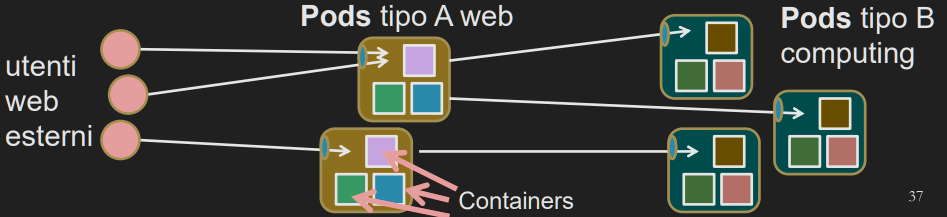
\includegraphics[keepaspectratio]{images/image2.png}}}

{}

{\pandocbounded{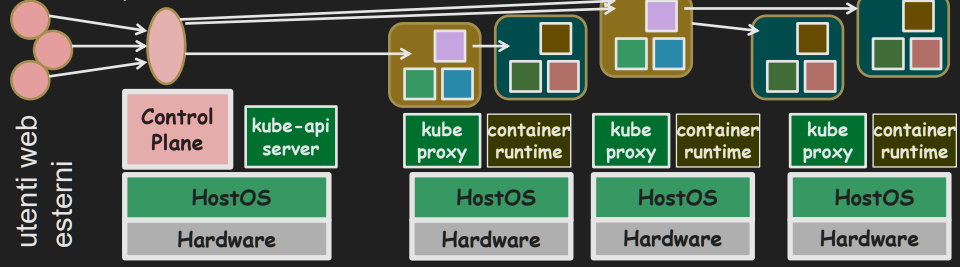
\includegraphics[keepaspectratio]{images/image4.png}}}

{}

{All'aumento del carico l'applicazione può configurare Kubernetes
affinchè faccia 3 operazioni:}

\begin{enumerate}
\tightlist
\item
  {Autoscaling verticale}{: aumento le risorse}{~(CPU, RAM,...) }{di un
  pod;}
\item
  {Autoscaling orizzontale}{: aumento repliche dei pods applicativi;}
\item
  {Cluster autoscaling:}{~aumento dei nodi che compongono il cluster
  ridistribuendo i pods. }
\end{enumerate}

{}

{Per realizzare questi autoscaling su host fisici occorre un sistema di
accensione host guidabile via software, per gli host virtuali occorre un
supporto che ci dia la possibilità di creare e configurare nuove VM in
automatico via software}

{}

{E\textquotesingle{} possibile creare un cluster kubernetes formato da
host che siano macchine virtuali, create manualmente su host fisici
oppure possono essere create via software (OpenSpace) su cloud pubblici
o privati.}

{}

{\pandocbounded{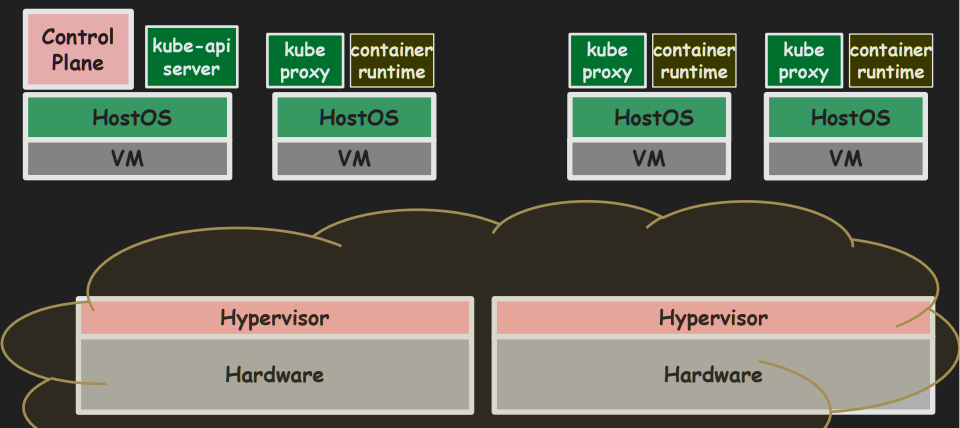
\includegraphics[keepaspectratio]{images/image6.png}}}

{}

{}

\subsubsection{\texorpdfstring{{Kubernetes-as-a-Service}}{Kubernetes-as-a-Service}}\label{h.yhr6y0xd3l43}

{Alcuni sistemi cloud offrono un servizio kubernetes senza che sia
necessario creare esplicitamente il cluster kubernetes, il cluster viene
creato ed installato dal provider cloud su richiesta e a chi produce
l\textquotesingle applicazione vengono fornite delle API mediante le
quali chiedere di inizializzare il cluster kubernetes e di dispiegarsi
sopra l\textquotesingle applicazione organizzata per kubernetes}{;
queste API però sono diverse fra servizi cloud.}

{}

\subsubsection{\texorpdfstring{{Container-as-a-Service}}{Container-as-a-Service}}\label{h.o28cy4xmuqsa}

{I sistemi cloud permettono di far eseguire un container, la cui
immagine è fornita dallo sviluppatore dell\textquotesingle applicazione,
in molteplici istanze su un cluster kubernetes-as-a-service costruito
nascostamente dal provider stesso. }

{Il container viene incapsulato in un pod predisposto dal provider cloud
ed eseguito nel cluster kubernetes.}

{}

{}

\section{\texorpdfstring{{DOCKER}}{DOCKER}}\label{h.3ppurwji5q6q}

{}

\subsection{\texorpdfstring{{Info
generali}}{Info generali}}\label{h.v2hul8flyw5j}

{Esistono tre componenti essenziali:}

{}

\begin{itemize}
\tightlist
\item
  {Docker Engine}{: si interfaccia con Linux e utilizza API per lavorare
  con il ciclo di vita dei containers {[} }{provides the core
  capabilities of managing containers}{~{]};}
\end{itemize}

{}

\begin{itemize}
\tightlist
\item
  {Docker Tools}{: insieme di funzioni a linea di comando che permettono
  di parlare con le API esposte dal componente precedentemente citato.
  Comandi utili per far partire container, creare loro immagini e
  configurare memoria e reti;}
\end{itemize}

{}

\begin{itemize}
\tightlist
\item
  {Docker Registry}{: dove le immagini dei container sono salvate con
  tags e versioni differenti.}
\end{itemize}

{}

{docker info =\textgreater{} mostra i dettagli del Docker Engine}

{}

{docker version=\textgreater{} mostra i dettagli del Docker Tools (+
Engine)}

{}

\subsection{\texorpdfstring{{Installazione}}{Installazione}}\label{h.awewb2eontor}

{Prima di procedere si necessita un }{s.o.}{~}{LUbuntu e}{~un account
Docker Hub.}

\begin{enumerate}
\tightlist
\item
  {Installare curl: ~ ~}{sudo apt-get update}
\end{enumerate}

{~ ~ ~ ~ ~ ~ ~ ~ ~ ~ ~ ~ ~ ~ ~ ~ ~ ~ ~ ~ ~ ~ ~ ~ sudo apt-get install
curl}

{}

\begin{enumerate}
\setcounter{enumi}{1}
\tightlist
\item
  {Installare docker engine: }{curl -fsSL https://get.docker.com -o
  get-docker.sh}
\end{enumerate}

{~ ~ ~ ~ ~ ~ ~ ~ ~ ~ ~ ~ ~ ~ ~ ~ ~ ~ ~ ~ ~ ~ sudo sh get-docker.sh}

{}

\begin{enumerate}
\setcounter{enumi}{2}
\tightlist
\item
  {Aggiungere l'utente in uso fra i sudoers {[}evitando di dover usare
  sempre sudo prima dei comandi{]}: }{~sudo usermod -aG docker
  \$\{USER\}}
\end{enumerate}

{~ ~ ~ ~ ~ ~ ~ ~ ~ ~ ~ ~ ~ ~ ~ ~ ~ ~ ~ ~ ~ ~ ~ ~ ~ ~ ~ ~id -nG
}{{[}controllo lista sudoers{]}}

{~ ~ ~ ~ ~ ~ ~ ~ ~ ~ ~ ~ ~ ~ ~ ~ ~ ~ ~ ~ ~ ~ ~ ~ ~ ~ ~ ~su -
\$\{USER\}}{~{[}Ricarico utente{]}}

{}

\subsection{\texorpdfstring{{Comandi
Docker}}{Comandi Docker}}\label{h.z0urwcbr7pqf}

{Sintassi generale: }{docker {[}option{]} {[}command{]} {[}arguments{]}}

{Usando il comando: `docker' posso controllare tutti i sottocomandi.}

{}

\subsection{\texorpdfstring{{Docker images e
container}}{Docker images e container}}\label{h.apoi1uqrh76t}

{I container docker sono creati tramite immagini docker che normalmente
vengono prese da Docker Hub, un portale dove tutti possono condividere
le proprie immagini Docker; per scaricare queste immagini usiamo il
comando:}

{~``}{docker run {[}images name{]}}{''.}

{Il comando cerca prima l'immagine in locale e se non la trova la
scarica, poi Docker crea un container dall'immagine ed esegue
l'applicazione al suo interno; l'immagine è copiata in uno spazio
locale.}

{Con il seguente comando invece otteniamo la possibilità di interagire
con il container tramite shell:}

{~``}{docker run -it {[}images name{]}}{''.}

{Se inseriamo, dopo `-it', anche }{- -name}{~seguito da una stringa
daremo un un nome custom al container.}

{}

\subsubsection{\texorpdfstring{{Ricerca e
Download}}{Ricerca e Download}}\label{h.jnulye2h3fue}

{Per cercare immagini su Docker Hub si usa:}

{~``}{docker search {[}images name{]}}{''.}

{Il ritorno del comando sarà una lista delle immagini con il nome
combacia con quello inserito nel comando (le immagini ufficiali avranno
il flag }{{[}OK{]}}{~sotto la voce }{OFFICIAL)}{~per scaricare:}

{~``}{docker pull {[}images name{]}}{''.}

{}

\subsubsection{\texorpdfstring{{Eliminazione}}{Eliminazione}}\label{h.9o4n5zq2mqkf}

{Per rimuovere le immagini scaricate si usa il comando:}

{~``}{docker }{rmi}{~{[}images name1{]} {[}images name2{]} {[}images
name N{]}}{''.}

{}

{Per rimuovere i container si usa il comando:}

{~``}{docker }{rm}{~{[}container name{]} or {[}container ID{]}}{''.}

{}

\subsubsection{\texorpdfstring{{Lavorare dentro i
container}}{Lavorare dentro i container}}\label{h.lxt1x6tzd8bo}

{Inserendo `}{-it}{' (come visto prima) nel comando run potremmo
inserire comandi dentro il container e quindi usare la shell per fare
operazioni dentro di esso.}

{In questo caso non è necessario il prefisso sudo}

{}

\subsubsection{\texorpdfstring{{Gestione}}{Gestione}}\label{h.koc6458ioaot}

{Per la gestione dei container esistono diversi comandi:}

{}

\begin{itemize}
\tightlist
\item
  {docker ps}{~=\textgreater{} mostra i container attivi, con ` }{-a }{'
  alla fine del comando possiamo visionare anche quelli inattivi
  (inserendo `}{-q}{' mostriamo solo gli ID);}
\end{itemize}

{}

\begin{itemize}
\tightlist
\item
  {docker ps -l }{~=\textgreater{} mostra i container più recente;}
\end{itemize}

{}

\begin{itemize}
\tightlist
\item
  {docker stop {[}container name{]} or {[}container
  ID{]}}{~=\textgreater{} ferma i container in esecuzione;}
\end{itemize}

{}

\begin{itemize}
\tightlist
\item
  {docker start {[}container name{]} or {[}container
  ID{]}}{~=\textgreater{} fa ripartire un container, con ` }{-ia}{~`
  dopo lo start possiamo usare i canali STDIN e STDOUT.}
\end{itemize}

{}

\begin{itemize}
\tightlist
\item
  {docker commit {[}container ID{]} {[}new image name{]}
  }{=\textgreater{} salva lo stato del container in una nuova immagine}
\end{itemize}

{}

{}

\subsection{\texorpdfstring{{Networks}}{Networks}}\label{h.h3bzngxffdw4}

{Quando creo un container in automatico viene creata
un\textquotesingle interfaccia di rete del container; oppure è possibile
indicare quale tipo di interfaccia di rete vogliamo mettere nel
container (dipendono dal tipo di driver).}

{Per funzionare è necessario avere dei driver specifici, alcuni già
presenti sono: }

{}

\begin{itemize}
\tightlist
\item
  {bridge}{:}{~}{inserito di default in ogni container, consente di
  comunicare con l\textquotesingle host e comunicare con
  l\textquotesingle esterno}{;}
\end{itemize}

{}

\begin{itemize}
\tightlist
\item
  {host}{: consente ad un container di utilizzare
  l\textquotesingle interfaccia di rete della macchina host come se
  fossero sue, però così facendo vado a perdere
  l\textquotesingle isolamento del container verso
  l\textquotesingle esterno;}
\end{itemize}

{~}

\begin{itemize}
\tightlist
\item
  {overlay}{:}{~}{connette più Docker }{deamons}{~insieme e permette di
  comunicare fra loro}{;}
\end{itemize}

{}

\begin{itemize}
\tightlist
\item
  {macvlan}{:}{~permette di assegnare un indirizzo MAC ad un container,
  rendendolo agli occhi di tutti un device fisico (utile per lavorare
  con le legacy application che si aspettano di essere connesse ad una
  rete fisica)}{;}
\end{itemize}

{~}

\begin{itemize}
\tightlist
\item
  {none}{: disabilita tutti i networking}{;}
\end{itemize}

{~}

\begin{itemize}
\tightlist
\item
  {custom network plugins}{.}
\end{itemize}

{}

{}

{- -networks =\textgreater{} per assegnare uno di questi driver ad un
container}

{}

{}

{Un }{bridge network}{~permette ai container connessi allo stesso bridge
di comunicare, isolando coloro non connessi.}

{}

{Le }{docker embedded DNS server}{~permettono la risoluzione dei nomi
per container connessi alla stessa network.}

\subsection{\texorpdfstring{{Compose}}{Compose}}\label{h.hk6jpwwyn477}

{Docker compose serve per scrivere un documento di tipo YML per creare }

{delle applicazioni costituite da più container; lo strumento originario
si }

{chiama docker-compose ed è un comando installato separatamente rispetto
a }

{docker.}

\subsection{\texorpdfstring{{DockerFile}}{DockerFile}}\label{h.3x53fpkri4bo}

{È uno script che contiene un'insieme di comandi e istruzioni che
vengono eseguite automaticamente nell'ambiente di docker per creare
nuove immagini; sotto si elencano alcuni di questi comandi.}

{}

\subsubsection{\texorpdfstring{{Comandi}}{Comandi}}\label{h.6y2j3jnxveht}

{}

\begin{itemize}
\tightlist
\item
  {FROM}{~=\textgreater{} ~indica l'immagine da dove bisogna creare
  un'immagine tutta nuova;}
\end{itemize}

{}

\begin{itemize}
\tightlist
\item
  {MAINTAINER}{~=\textgreater{} contiene il nome di chi ``mantiene''
  l'immagine;}
\end{itemize}

{}

\begin{itemize}
\tightlist
\item
  {RUN}{~=\textgreater{} esegue un comando durante la build;}
\end{itemize}

{}

\begin{itemize}
\tightlist
\item
  {COPY}{~=\textgreater{} copia un file dall'host alla nuova immagine;}
\end{itemize}

{}

\begin{itemize}
\tightlist
\item
  {ADD}{~=\textgreater{} come il precedente ma è possibile mettere anche
  un URL come sorgente;}
\end{itemize}

{}

\begin{itemize}
\tightlist
\item
  {ENV}{~=\textgreater{} definisce una variabile di ambiente
  utilizzabile in altri ambienti;}
\end{itemize}

{}

\begin{itemize}
\tightlist
\item
  {CMD}{~=\textgreater{} esegue un comando quando si costruisce un nuovo
  container dall'immagine docker;}
\end{itemize}

{}

\begin{itemize}
\tightlist
\item
  {ENTRYPOINT}{~=\textgreater{} il comando di default da fare quando il
  container è in esecuzione;}
\end{itemize}

{}

\begin{itemize}
\tightlist
\item
  {WORKDIR}{~=\textgreater{} indica dove fare i comandi fatti con
  `CMD';}
\end{itemize}

{}

\begin{itemize}
\tightlist
\item
  {USER}{~=\textgreater{} ;}
\end{itemize}

{}

\begin{itemize}
\tightlist
\item
  {VOLUME}{~=\textgreater{} ;}
\end{itemize}

{}

{}

\subsection{\texorpdfstring{{Docker
Swarm}}{Docker Swarm}}\label{h.v458pgb2juyv}

{Permette di utilizzare un'applicazione fatta da container su più
macchine (fisiche o virtuali), l\textquotesingle insieme di macchine (o
nodi) si chiama SWARM, dove un nodo che prende il nome di manager
gestisce l'insieme.}

{}

{docker swarm init =\textgreater{} per scegliere il manager}

{}

{Lo swarm può lanciare degli stack (gruppo di servizi), dove ogni
servizio è lo stesso visto nel Compose ( un'immagine di container e le
proprie strutture). Ogni stack ~è composto da tanti task (ogni
}{istanza}{~di un container) e il manager gestisce le richieste fra
task.}

{\pandocbounded{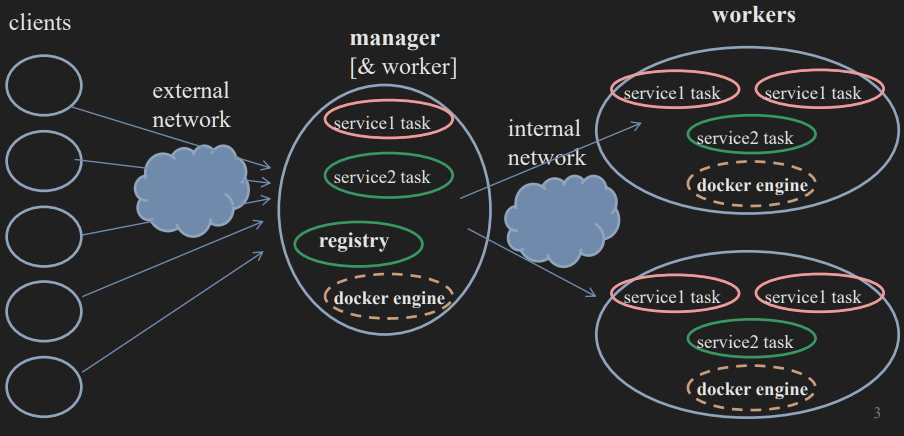
\includegraphics[keepaspectratio]{images/image5.png}}}

{In essence, a stack is a set of tasks (working containers), grouped in
services, running over a cluster of worker nodes and coordinated by a
manager node.}

{}

{}

{}

{}

\subsection{\texorpdfstring{{Kubernetes}}{Kubernetes}}\label{h.r0gopwkqfyte}

{Kubernetes è un\textquotesingle architettura software con una struttura
client-server che esegue su un cluster (cioè un gruppo di host) una
applicazione. }

{L\textquotesingle interfacciamento dell\textquotesingle amministratore
di kubernetes avviene tipicamente mediante un client.}

{Si può gestire bene la scalabilità dell'applicazione e rispetto a swarm
c'è una organizzazione maggiore fra container grazie ai }{pods}{.}

{I pods sono un' insieme di più container con caratteristiche simili
(stessi indirizzi ip, stesso spazio di porte) che comunicano fra loro
come se fossero sulla stessa macchina fisica.}

{Un insieme di istanze dello stesso pod (repliche) è detto deployments.}

{}

{I pods}{~sono classificati con }{label}{, stringhe di nomi + valori,
ugual label ugual funzionalità.}

{Per ricercare una risorsa invece si utilizza il }{selectors}{, andando
a specificare una determinata label.}

\subsubsection{\texorpdfstring{{Services}}{Services}}\label{h.6npj56aravbd}

{Un servizio è un insieme di pods individuati da un selettore, il
servizio tipicamente include anche la politica con cui viene effettuato
il bilanciamento di carico delle richieste tra i diversi pods di quello
stesso servizio.}

{\pandocbounded{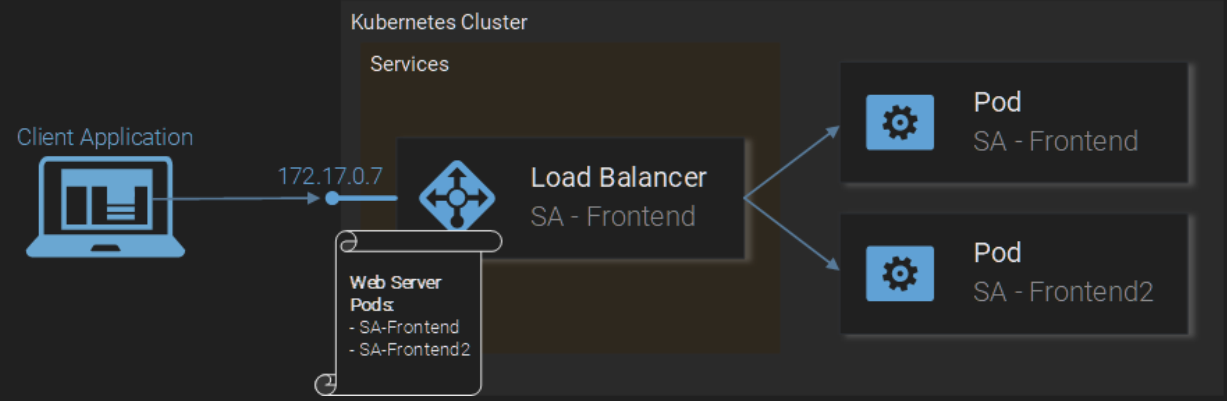
\includegraphics[keepaspectratio]{images/image1.png}}}

{}

\subsubsection{\texorpdfstring{{Autoscaling}}{Autoscaling}}\label{h.i7mlgya9xhn4}

{Tecnica che incrementa e/o riduce in modo dinamico l'ammontare di
risorse a disposizione di una o più server farm.}

{In kubernetes si utilizza quando all'aumentare di richieste per dei
servizi si necessita di più }{pod.}

{}

{}

{}

{}

{}

\section{\texorpdfstring{{BASH}}{BASH}}\label{h.8hjqojdwwuad}

{}

\subsection{\texorpdfstring{{Permessi}}{Permessi}}\label{h.7lacb1x7k66c}

{Ogni file ha un proprietario ed un gruppo del proprietario, il
proprietario/creatore poi può cambiare il proprietario del file con il
comando:}

{chown }{{[}nuovoProprietario{]}}{~{[}nomeFile{]}}

{}

{il gruppo:}

{chgrp }{{[}nuovoGruppo{]}}{~{[}nomeFile{]}}

{i premessi::}

{chmod }{{[}numeriDeiPermessi{]}}{~{[}nomeFile{]}}

{}

{}

{Ciascun file mantiene diversi diritti di lettura, scrittura ed
esecuzione assegnati al proprietario, al gruppo del proprietario e a
tutti gli altri:}

{}

\begin{itemize}
\tightlist
\item
  {Lettura (valore 4, simbolo r);}
\end{itemize}

{}

\begin{itemize}
\tightlist
\item
  {Scrittura (valore 2, simbolo w);}
\end{itemize}

{}

\begin{itemize}
\tightlist
\item
  {Esecuzione (valore 1, simbolo x);}
\end{itemize}

{}

{Quindi se voglio, per esempio, mettere che tutti possono fare tutto su
quel file devo fare:}

{chmod 777 {[}nomeFile{]}}

{questo perché il 1° sette indica scrittura, lettura e esecuzione
all'user (4+2+1), il 2° sette indica gli stessi permessi al gruppo e il
3° }{sette}{~indica i permessi di tutti gli altri.}

{\pandocbounded{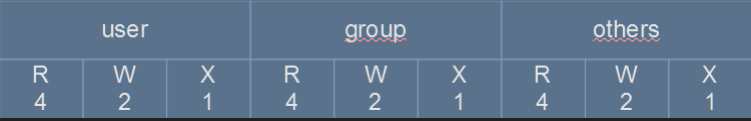
\includegraphics[keepaspectratio]{images/image7.png}}}

\subsection{\texorpdfstring{{Caratteri con utilizzi
speciali}}{Caratteri con utilizzi speciali}}\label{h.45juy67n4iep}

{}

\begin{itemize}
\tightlist
\item
  {; }{~-> ~separatore tra comandi , che stabilisce cioè dove finisce un
  comando e dove inizia il successivo;}
\end{itemize}

{}

\begin{itemize}
\tightlist
\item
  {\textbackslash{} }{~-> carattere di escape, ferma l'interpretazione di
  alcuni caratteri speciali;}
\end{itemize}

{}

\begin{itemize}
\tightlist
\item
  {``...'' }{-> tutto ciò che è scritto al suo interno viene letto in
  maniera letterale;}
\end{itemize}

{}

\begin{itemize}
\tightlist
\item
  {* ? {[}\ldots{]} ~}{-> sono caratteri che vengono inseriti dall'utente
  nei comandi digitati e che la shell interpreta cercando di sostituirli
  con una sequenza di caratteri; possono essere sostituiti con:}
\end{itemize}

\begin{enumerate}
\tightlist
\item
  {* :una qualunque sequenza di caratteri;}
\item
  {? :un solo e unico carattere;}
\item
  {{[}...{]} :un solo carattere tra quelli specificati in un elenco
  scritto all'interno dei caratteri.}
\end{enumerate}

{}

\begin{itemize}
\tightlist
\item
  {\textless{}}{~-> riceve input da file;}
\end{itemize}

{}

\begin{itemize}
\tightlist
\item
  {\textgreater{} }{-> mandare std output verso file eliminando il
  vecchio contenuto del file;}
\end{itemize}

{}

\begin{itemize}
\tightlist
\item
  {\textgreater\textgreater{} }{-> mandare std output verso file
  aggiungendolo al vecchio contenuto del file;}
\end{itemize}

{}

\begin{itemize}
\tightlist
\item
  {\textbar{} }{-> redirige l\textquotesingle output di un programma
  nell' input di un altro programma;}
\end{itemize}

{}

\begin{itemize}
\tightlist
\item
  {\textless\textless{}}{parolaFine}{~}{-> redirige tutto da dopo il
  metacarattere alla prossima apparizione della keyword }{parolaFine}{;}
\end{itemize}

{}

\begin{itemize}
\tightlist
\item
  {\textless\textless\textless{}}{parolaFine}{~}{-> viene ridirezionato
  nell\textquotesingle input la parola che compare subito dopo il
  metacarattere;}
\end{itemize}

{}

\begin{itemize}
\tightlist
\item
  {}
\end{itemize}

{}

{}

{}

{}

\subsection{\texorpdfstring{{Esecuzione
script}}{Esecuzione script}}\label{h.msnbjeuypgoj}

{Normalmente, se una shell lancia uno script, questo viene eseguito in
una subshell e le modifiche fatte su variabili non vengono viste dal
padre.}

{È possibile però che una shell possa eseguire uno script senza
creazione di subshell, per farlo basta usare il comando:}

{}

{source}{~}{nomeScript}{~}

{oppure}

{}

{. ~}{~}{nomeScript}

{}

{Se però invochiamo con source uno script}{~che necessita}{~di un
}{interprete diverso}{~provochiamo dei problemi, poiché }{non verrà
lanciato l\textquotesingle interprete corretto }{indicato nella prima
riga dello script.}

\subsection{\texorpdfstring{{Comandi}}{Comandi}}\label{h.q7fep3v91n2i}

\subsubsection{\texorpdfstring{{Set}}{Set}}\label{h.dx2a94e7s5il}

{Se il comando viene lanciato }{senza parametri}{~visualizza tutte le
variabili della shell}{, altrimenti lanciato }{con parametri}{~serve a
}{settare o resettare un\textquotesingle opzione di comportamento della
shell}{~in cui viene lanciato.}

\subsubsection{\texorpdfstring{{Echo}}{Echo}}\label{h.ultvyv6feag4}

{Stampa quello che si scrive dopo il comando.}

\subsubsection{\texorpdfstring{{Mkdir/Rmdir}}{Mkdir/Rmdir}}\label{h.temawjp7mx6y}

{Crea/elimina una directory nel percorso specificato.}

\subsubsection{\texorpdfstring{{Cat}}{Cat}}\label{h.na34hz2wfgir}

{Visualizza in output il contenuto del file specificato.}

\subsubsection{\texorpdfstring{{Env}}{Env}}\label{h.ftgv9yksgljz}

{Visualizza tutte le variabili e i loro valori.}

\subsubsection{\texorpdfstring{{Which}}{Which}}\label{h.gapcjj5hdjx}

{Visualizza il percorso in cui si trova (solo se nella PATH)
l'eseguibile.}

\subsubsection{\texorpdfstring{{Sed}}{Sed}}\label{h.7rz3gslfum6k}

{Il comando è così strutturato:}

{sed}{~`}{s}{/es1/es2/}{g}{' nomeFile}

{In questo modo per ogni riga processata (senza }{g}{~solo la prima)
}{es1}{~verrà sostituito con }{es2}{.}

{}

{}

{}

{}

{}

{}

{}

\section{\texorpdfstring{{DOMANDE}}{DOMANDE}}\label{h.y4gl3bst2hll}

{}

\subsection{\texorpdfstring{{Parte 1}}{Parte 1}}\label{h.q1i6nkap762d}

\begin{enumerate}
\tightlist
\item
  {Un container in ambiente linux in cui esegue un web server, può
  essere considerato un "micro-servizio"?. Motivare la risposta. }
\end{enumerate}

{}

{Si, un container Linux che ospita un web server può rappresentare uno
dei microservizi di un\textquotesingle applicazione più ampia}

{}

{}

\begin{enumerate}
\setcounter{enumi}{1}
\tightlist
\item
  {Citare i due modi mediante i quali si risolve il problema delle
  istruzioni privilegiate nella full-virtualization. }
\end{enumerate}

{}

{Per eseguire le istruzioni in kernel mode (ring 0) si usano le seguenti
tecniche:}

\begin{itemize}
\tightlist
\item
  {Binary translation}{: si riscrivono a run-time le parti del codice
  del s.o.guest che dovrebbero essere eseguite in modo privilegiato.}
\end{itemize}

{}

\begin{itemize}
\tightlist
\item
  {Hardware assisted}{: viene aggiunto un nuovo ring chiamato }{ring
  -1}{, il sistema host e l'hypervisor vengono eseguiti in quest'ultimo
  ring mentre il guest in quello 0 (esecuzione di istruzioni
  privilegiate sotto il controllo dell'hypervisor).}
\end{itemize}

{}

{}

{}

\begin{enumerate}
\setcounter{enumi}{2}
\tightlist
\item
  {In una macchina fisica in cui è installato Docker, a cosa serve il
  docker registry?}
\end{enumerate}

{}

{Componente essenziale di un docker, è dove le immagini dei container
sono salvate con tags e versioni differenti.}

{}

{}

\begin{enumerate}
\setcounter{enumi}{3}
\tightlist
\item
  {Posso mettere in esecuzione due container, partendo dalla stessa
  immagine, in modo che i due container }{eseguano}{~simultaneamente ?
  Potrebbero generarsi interferenza tra i due container? Motivare la
  risposta. }
\end{enumerate}

{}

{È possibile eseguire due container dalla stessa immagine
contemporaneamente e non dovrebbero generarsi problemi essendo i
container creati per rimanere isolati e lavorare in autonomia.}

{~~~~~~~~}

{}

\begin{enumerate}
\setcounter{enumi}{4}
\tightlist
\item
  {Supponiamo che un immagine di un container contenga tutto il
  necessario per eseguire un applicativo, ad esempio il database
  documentale }{mongo.}{~Però in quell\textquotesingle immagine non è
  installato un altro applicativo, ad esempio il magnifico editor
  testuale vim. L\textquotesingle applicativo vim è però installato nel
  sistema operativo Linux della macchina fisica. Supponiamo di mettere
  in esecuzione un container partendo da quell\textquotesingle immagine.
  Posso eseguire, all\textquotesingle interno del container,
  l\textquotesingle applicativo vi? Motivare la risposta}
\end{enumerate}

{}

{Si, i container possono utilizzare gli stessi servizi del s.o. host.}

{}

{}

\begin{enumerate}
\setcounter{enumi}{5}
\tightlist
\item
  {A cosa serve il comando docker build ? }
\end{enumerate}

{}

{Il comando docker build è utilizzato per creare
un\textquotesingle immagine Docker a partire}

{da un Dockerfile; permette di definire in modo dichiarativo tutte le ~
}

{configurazioni e le dipendenze necessarie per
l\textquotesingle esecuzione dell\textquotesingle applicazione ~}

{all\textquotesingle interno del container.}

{}

\begin{enumerate}
\setcounter{enumi}{6}
\tightlist
\item
  {Posso salvare l\textquotesingle immagine di un container in
  esecuzione, dopo averlo }{stoppato?}{~Se ritenete che si possa, quale
  comando dovreste usare?}
\end{enumerate}

{}

{Si, dopo aver stoppato il container con }{docker stop}{~possiamo
salvare l'immagine in una nuova con }{docker commit {[}id container{]}
{[}nuovo nome immagine{]}}{.}

{}

{}

{}

{}

\begin{enumerate}
\setcounter{enumi}{7}
\tightlist
\item
  {Che tipo di servizio offre il docker hub (https://hub.docker.com/) ?}
\end{enumerate}

{}

{~ ~ ~ ~ ~ ~Docker Hub è un servizio di registro di container pubblico
fornito da Docker. ~}

{~ ~ ~ ~ ~ ~Offre una piattaforma centralizzata per la condivisione, la
distribuzione e la }

{~ ~ ~ ~ ~ ~collaborazione sulle immagini Docker.}

{}

{}

\begin{enumerate}
\setcounter{enumi}{8}
\tightlist
\item
  {Un container offre un servizio sulla propria porta TCP 80. Nella
  macchina fisica in cui voglio eseguire il container, quella porta 80 è
  usata da un\textquotesingle altra applicazione. Senza modificare il
  container, posso eseguire quel container in modo da esporre il
  servizio offerto dal container su una diversa porta nella macchina
  fisica, ad esempio la porta 60000? Motivare la risposta.}
\end{enumerate}

{}

{Sì è possibile, infatti il comando }{docker run}{~può contenere tanti
parametri, fra questi c'è il }{-p}{~che permette di decidere in quale
porta fisica (60000) deve essere mappata la porta del container (80).}

{}

{}

\begin{enumerate}
\setcounter{enumi}{9}
\tightlist
\item
  {A cosa serve un Dockerfile ?}
\end{enumerate}

{}

{~ ~ ~ ~ ~ È uno script che contiene un'insieme di comandi e istruzioni
che vengono}

{~ ~ ~ ~ ~ eseguite automaticamente nell'ambiente di docker per creare
nuove immagini}

{}

{}

\begin{enumerate}
\setcounter{enumi}{10}
\tightlist
\item
  {~Quale è la principale funzionalità che viene messa a disposizione
  dal DNS embedded che docker automaticamente configura per i container
  che usano una stessa user-defined bridge network?}
\end{enumerate}

{}

{Il DNS embedded permette la risoluzione dei nomi per container connessi
}{alla}{~}{stessa}{~network.}

{}

{}

\begin{enumerate}
\setcounter{enumi}{11}
\tightlist
\item
  {E\textquotesingle{} possibile attaccare un container a più di una
  rete?}
\end{enumerate}

{}

{Sì, è possibile attaccare un container a quante reti si voglia basta
che usino differenti driver.}

{}

{}

\begin{enumerate}
\setcounter{enumi}{12}
\tightlist
\item
  {Che cos\textquotesingle è iptables/netfilter ?}
\end{enumerate}

{}

{Iptables: è un comando (un eseguibile binario) che prende come
argomenti }

{dei comandi con cui si definiscono delle regole che sono realizzate da
più }

{moduli del kernel linux;}

{}

{Netfilter: è un insieme di moduli del kernel linux che lavorano su }

{pacchetti di rete.}

{}

{}

\begin{enumerate}
\setcounter{enumi}{13}
\tightlist
\item
  {Che cos\textquotesingle é docker-compose e a cosa serve ?}
\end{enumerate}

{}

{È uno strumento che permette la creazione di applicazioni con più
container, la loro rimozione e il loro controllo in modo coordinato.}

{}

{}

\begin{enumerate}
\setcounter{enumi}{14}
\tightlist
\item
  {Nel contesto di docker swarm, qual\textquotesingle è la differenza
  tra un nodo manager ed un nodo worker?}
\end{enumerate}

{}

{il nodo manager oltre a gestire gli altri nodi (worker) e distribuire i
task fra loro riceve anche le richieste dai client esterni e le
distribuisce ai vari servizi.}

{Il nodo worker invece (anche il manager lo è) contiene le repliche
(task di servizi) di un servizio ed è responsabile dell'esecuzione dei
container all'interno del cluster}

{}

{}

\begin{enumerate}
\setcounter{enumi}{15}
\tightlist
\item
  {Nel contesto di docker swarm, che cos\textquotesingle è uno stack? }
\end{enumerate}

{}

{Uno stack è un gruppo di task, dove ogni task è un container in
esecuzione.}

{}

{}

\begin{enumerate}
\setcounter{enumi}{16}
\tightlist
\item
  {Nel contesto di kubernetes, che cosa sono i pods ?}
\end{enumerate}

{}

{I pods sono un' insieme di più container con caratteristiche simili
(stessi indirizzi ip, stesso spazio di porte) che comunicano fra loro
come se fossero sulla stessa macchina fisica.}

{~}

{}

\begin{enumerate}
\setcounter{enumi}{17}
\tightlist
\item
  {Nel contesto di kubernetes, qual\textquotesingle è la differenza tra
  deployments e services?}
\end{enumerate}

{~~~~~~~~}

{~~~~~~~~Un deployments è un insieme di repliche dello stesso pod, un
services è }

{sempre un insieme di pods ma individuati da un selettore ed è indicato
anche come accedere ai seguenti pod e le politiche di bilanciamento; in
sostanza prima si istanziano i deployments poi davanti a ciascun
deployments si istanza il servizio che ne regola l'accesso..}

{~~~~~~~~}

{}

\begin{enumerate}
\setcounter{enumi}{18}
\tightlist
\item
  {Quale è la principale differenza che distingue le connessioni
  stabilite mediante l\textquotesingle ausilio di un server STUN
  rispetto a quelle connessioni che hanno
  }{richieste}{~l\textquotesingle utilizzo di un server TURN? }
\end{enumerate}

{}

{}

{}

{}

\begin{enumerate}
\setcounter{enumi}{19}
\tightlist
\item
  {A cosa serve il protocollo TURN?}
\end{enumerate}

{}

{}

{}

\subsection{\texorpdfstring{{Parte 2}}{Parte 2}}\label{h.lx0jsvh85x20}

\begin{enumerate}
\tightlist
\item
  {Spiegare la differenza tra virtualizzazione della CPU e Emulazione
  della CPU.}
\end{enumerate}

{}

{Con la virtualizzazione della cpu in un host si crea una CPU virtuale
che esegue lo stesso tipo di istruzioni macchina della CPU reale. La CPU
virtuale quindi può fare eseguire le istruzioni dei programmi
direttamente dalla CPU reale. Con l'emulazione della cpu, invece, in un
host si costruisce una CPU virtuale che esegue istruzioni di tipo
diverso da quello della CPU reale, ad esempio si vuole creare una CPU
virtuale di tipo x86-64 che operi però su un processore reale della
famiglia ARM a 64 bit. In tal caso, le istruzioni dei programmi che
operano nella macchina virtuale sono istruzioni macchina per processori
della famiglia x86-64 e tali istruzioni non possono essere eseguite
sulla CPU reale, quindi devono essere tradotte in istruzioni macchina
per ARM a 64 bit e queste saranno eseguite. }

{}

{}

{}

\begin{enumerate}
\setcounter{enumi}{1}
\tightlist
\item
  {Cos\textquotesingle è kubernetes e a cosa serve?}
\end{enumerate}

{}

{Kubernetes è un sistema che prevede di scrivere applicazioni formate da
servizi implementati mediante dei pods. Un pod è un gruppo di container
che operano tra loro come se si trovassero su una stessa macchina
fisica. Kubernetes consente che questi pods vengano dispiegati in un
cluster di macchine gestito da un nodo manager. Un servizio può
replicare i propri pod anche dinamicamente, allo scopo di gestire la
scalabilità e la resilienza dell'applicazione, in caso di variazione del
numero di richieste e in caso di fault di alcuni pods}

{}

{}

{}

\begin{enumerate}
\setcounter{enumi}{2}
\tightlist
\item
  {Nel contesto di kubernetes, i container che appartengono ad uno
  stesso pod hanno lo stesso indirizzo IP ?}
\end{enumerate}

{}

{Si, i container che appartengono ad uno stesso pod hanno lo stesso
indirizzo IP poiché sono strutturati per vedersi come se appartenessero
ad una stessa macchina, in tal modo si facilitano le comunicazioni tra i
container di uno stesso host poiché ciascun container può raggiungere i
container del suo stesso pod mediante il localhost. }

{}

{}

\begin{enumerate}
\setcounter{enumi}{3}
\tightlist
\item
  {~Nel contesto di kubernetes, se ho una applicazione in cui alcuni
  suoi pods sono replicati, i container che appartengono ad uno stesso
  pod hanno lo stesso indirizzo IP? Motivare la risposta}
\end{enumerate}

{}

{Si, i container di uno stesso pod continuano ad avere lo stesso
indirizzo IP, ma i container che appartengono a repliche diverse di uno
stesso tipo di pod ovviamente hanno indirizzi diversi.}

{}

{}

\begin{enumerate}
\setcounter{enumi}{4}
\tightlist
\item
  {Una stessa immagine di un container, può essere usata per mettere in
  esecuzione un container su due host diversi, uno con un Linux che
  opera su un processore AMD a 64 bit, e l\textquotesingle altro con un
  Linux che opera su un processore ARM a 64 bit? Motivare la risposta.}
\end{enumerate}

{}

{NO!!!!! Non è possibile perché gli eseguibili binari di quel container
contengono istruzioni macchina di un certo tipo (per una certa famiglia
di processori, ad esempio AMD o ARM) e quelle istruzioni non possono
essere eseguite su un processore diverso.}

{}

{~}

{}

\begin{enumerate}
\setcounter{enumi}{5}
\tightlist
\item
  {Nel contesto della bash, che cos\textquotesingle è un file descriptor
  ?}
\end{enumerate}

{}

{Un file descriptor è un\textquotesingle astrazione che rappresenta
univocamente un file aperto da un certo processo. Nella sostanza un file
descriptor è un numero intero, maggiore o uguale a zero, che costituisce
un indice per indicare una riga di una tabella dei file aperti dal
processo. Quella riga indica a sua volta una riga in una tabella che
contiene le informazioni sui file aperti in tutto l'host. Quindi,
indirettamente, un file descriptor consente di ottenere ed usare
informazioni su un file aperto e di poter accedere a quel file. }

{}

{}

\begin{enumerate}
\setcounter{enumi}{6}
\tightlist
\item
  {E\textquotesingle{} possibile che due processi, contemporaneamente in
  esecuzione su uno stesso sistema operativo, abbiano lo stesso PID?
  E\textquotesingle{} possibile che due processi, in esecuzione su uno
  stesso sistema operativo ma in due momenti diversi, abbiano lo stesso
  PID? Motivare la risposta.}
\end{enumerate}

{}

{La risposta alla prima parte della domanda è NO. Due processi,
contemporaneamente in esecuzione su uno stesso sistema operativo devono
per forza avere PID DIVERSI perché quel PID deve identificare
UNIVOCAMENTE ciascuno dei processi attualmente in esecuzione. Però, al
termine dell'esecuzione di un processo, il PID di quel processo viene
rilasciato e potrebbe essere assegnato ad un diverso processo che
venisse messo in esecuzione in un secondo momento. Quindi la risposta
alla seconda parte della domanda è SI. }

{}

{}

\begin{enumerate}
\setcounter{enumi}{7}
\tightlist
\item
  {Qual\textquotesingle è la differenza tra un hypervisor di tipo
  bare-metal (tipo 1) ed uno di tipo hosted (tipo 2) ? }
\end{enumerate}

{}

{Un hypervisor di tipo bare-metal (tipo 1) si appoggia direttamente
sull'hardware e sostituisce completamente il sistema operativo. Invece,
un hypervisor di tipo hosted (tipo 2) si appoggia su un sistema
operativo esistente che a sua volta si appoggia sull'hardware.}

{}

{}

\begin{enumerate}
\setcounter{enumi}{8}
\tightlist
\item
  {Nei moderni processori, esiste un ring di protezione di valore -3 ?
  Motivare la risposta. }
\end{enumerate}

{}

{NO, non esiste un ring di protezione -3. L'unico ring di protezione con
indice negativo ha valore -1 ed è il ring di protezione che contiene le
funzionalità che l'HW mette a disposizione degli hypervisor per gestire
il problema delle istruzioni privilegiate e per poter gestire
contemporaneamente più macchine virtuali, anche annidate una dentro
l'altra. }

{}

{}

\begin{enumerate}
\setcounter{enumi}{9}
\tightlist
\item
  {Un file eseguibile binario ha questi permessi: 740 se io sono un
  utente che non è proprietario del file ma che appartiene allo stesso
  gruppo del file: posso eseguire quel file? Motivare la risposta. }
\end{enumerate}

{}

{NO, io non ho i diritti di eseguire quel file perché io su quel file ho
i diritti del gruppo, ovvero i diritti pari al valore 4, che rappresenta
la sola possibilità di lettura.}

{}

{}

\subsection{\texorpdfstring{{Esame 1}}{Esame 1}}\label{h.9by5o2qx7hz}

\begin{enumerate}
\tightlist
\item
  {~Comando source, cosa fa;}
\end{enumerate}

{}

{Risposta pers}{~}{{[}Errata{]}}{:}{~Indica dov\textquotesingle è
collocato un file all\textquotesingle interno della macchina, quindi
indica il suo percorso assoluto.}

{}

{}

\begin{enumerate}
\setcounter{enumi}{1}
\tightlist
\item
  {Operatore \textless\textless\textless{} in bash;}
\end{enumerate}

{}

{Risposta pers}{: }{Vuota}

{}

\begin{enumerate}
\setcounter{enumi}{2}
\tightlist
\item
  {Vertical pod autoscaling;}
\end{enumerate}

{}

{Risposta }{pers}{~}{{[}Ok ma incompleta, che tipo di
risorse?{]}}{:}{~}{il vertical pod autoscaling è quando si aumentano le
risorse ai pod perchè c\textquotesingle è una richiesta maggiore di un
servizio.}

{}

{}

\begin{enumerate}
\setcounter{enumi}{3}
\tightlist
\item
  {Un utente può appartenere a più gruppi? Fare esempi;}
\end{enumerate}

{}

{Risposta }{pers}{~{[}Ok{]}}{:}{~}{Sì,}{~è possibile che un un utente
appartenga a più gruppi. Per esempio può appartenere a vari gruppi
associati a dei file o a gruppi con vari permessi di amministratore, di
stampa, ecc.}

{}

{}

\begin{enumerate}
\setcounter{enumi}{4}
\tightlist
\item
  {Cos'è OpenStack;}
\end{enumerate}

{}

{Risposta pers}{~}{{[}Errata{]}}{: }{OpenStack è un programma che ci
permette di utilizzare docker swarm e gestire i vari nodi.}

{}

{}

\begin{enumerate}
\setcounter{enumi}{5}
\tightlist
\item
  {Cos'è uno stack in docker swarm;}
\end{enumerate}

{}

{Risposta }{pers}{~{[}Ok{]}}{:}{~}{Uno stack è
un\textquotesingle insieme di task.}

{}

\begin{enumerate}
\setcounter{enumi}{6}
\tightlist
\item
  {Fra i vari container dentro lo sesso pod docker swarm inserisce
  automaticamente un filesystem condiviso?}
\end{enumerate}

{}

{Risposta }{pers}{~{[}Ok{]}}{: }{No, il filesystem condiviso va inserito
manualmente.}

{}

\begin{enumerate}
\setcounter{enumi}{7}
\tightlist
\item
  {Cos'è un immagine di un container.}
\end{enumerate}

{}

{Risposta }{pers}{~{[}Ok{]}}{: }{l\textquotesingle immagine di un
container è un \textquotesingle file\textquotesingle{} che serve per
creare il container, indica com\textquotesingle è formato e cosa farà.
Con docker hub è possibile scaricarne di nuovi.}

{}

\end{document}
